\documentclass[../main.tex]{subfiles}
\begin{document}

\chapter{Introduction}
\labch{intro}

\section{The old nature-nurture debate}

Both genes and environment play a crucial role during the entire life of 
an organism, from development to senility, and in particular in the 
manifestation of complex diseases. Every phenotype arises as a 
consequence of the interactions of genes both with each other and with 
the environment. Other things being equal, genetic variation among 
individuals\autocite{Auton2015} results in phenotypic variation; on the 
other hand, environment can influence a trait as much as any gene, 
especially if the trait is \textit{complex}.

A complex trait, as opposed to a mendelian trait, is a phenotype whose 
variation in the population cannot be explained by the variation in a 
single gene. For instance, height is a complex trait as there have been 
found many loci contributing to it: each of them gives a small 
contribution, and the final height depends on the combination of all the 
alleles in the individual's genome. Clearly, not \textit{all} phenotypic 
variation in a population can be explained by genetic variation, for the 
environment has an effect as well. The proportion of phenotipic variance 
that can be explained by genetic variance is called heritability (see 
\refsec{heritability}), which for height is about 
80\%\autocite{Visscher2008a}. It cannot be said that an allele 
determines a phenotype, but rather variation at that locus can result in 
phenotypic variation (for instance disease status), under the influence 
of an appropriate environment.

Gradually, it happened that the focus moved from candidate genes to 
whole genomes. As a consequence of the large amount of genetic variation 
among individuals, larger sample sizes were needed to study variation at 
a population level, thus many laboratories decided to join their forces 
to create consortia.

One of the driving ideas of the Human Genome 
Project\autocite{Lander2001,Venter2001} was that the knowledge of the 
human genome sequence and its annotation would have helped to explain 
and cure diseases. Indeed, epigenetic markers aside, DNA is the only 
heritable molecule, therefore heritable traits must be related to it. In 
2005, a powerful method was developed in order to harness the huge 
amount of data collected from the sequencing of genomes: genome-wide 
association studies (see \refsec{gwas} for a technical description of 
the method), which find association between genetic variants and 
phenotypic traits, in the sense that people harbouring a particular 
allele might be more liable to develop a particular phenotype, and such 
liability can be quantified by an odds ratio (or effect size).

Another method to investigate complex traits is the mapping of loci that 
influence gene expression (see \refsec{eqtl}). Indeed, gene expression 
is an intermediate phenotype in the sense that it is one of the 
mechanistic steps that bring from a gene to an accomplished phenotype, 
therefore expression can be used as a proxy for the phenotype. In eQTL 
mapping, each SNP is assigned a coefficient according to how much the 
expression of a gene is altered by the presence of that SNP.

Environment can influence gene expression, and in fact also genes ---for 
instance, exposure to UV rays can cause mutations. However, since the 
effects of environment are difficult to quantify, much of the reaserch 
on complex traits and diseases was concerned on genetic factors. Here, 
our focus will be primarily on SNPs as genetic variants, and on humans 
as organisms of interest, with particular reference to their diseases.

\section{Genome-wide association studies and expression quantitative 
	trait loci mapping}

\marginnote{As of 2018-06-25, the GWAS Catalog contains 3420 
	publications and 62652 unique SNP-trait associations. 
	\url{https://www.ebi.ac.uk/gwas/home}}

The classical method to find associations between SNP and disease is the 
GWAS: several individuals in a cohort of cases and controls are 
genotyped, and the variants that occur more frequently in cases than in 
controls are said to be associated with the disease. Unless the full 
genome of the samples is sequenced, however, not every single variant in 
the population will be known, and in fact those that result associated 
to the disease are almost never the causal ones, but are only in linkage 
disequilibrium with the unknown causal SNP\autocite{Visscher2012}. 
Moreover, even if the causal variant were known, we still would not know 
much about the mechanism or the underlying biology of the disease, 
although it is possible to leverage a functional annotation of the 
genome to draw conclusions\sidenote{For instance, most 
	disease-associated SNPs fall in enhancers, as reported in a paper by 
	Ernst published in 2011, using data from the ENCODE project.}.

Despite these limitations, GWAS have revealed some interesting facts. 
First and foremost, complex traits are highly 
polygenic\autocite{Visscher2017}: there are many loci which, together, 
can carry a number of combination of alleles, each of which increases or 
decreases the probability of disease by a small amount. One of the 
hypothesis was that of \enquote{common disease, common variant}, but 
actually there can be few rare variants that contribute substantially to 
the disease risk, as well as many common variants with a small effect 
size. For some examples of success stories, see 
\reffig{introduction/gwas_success}.

\begin{figure}
	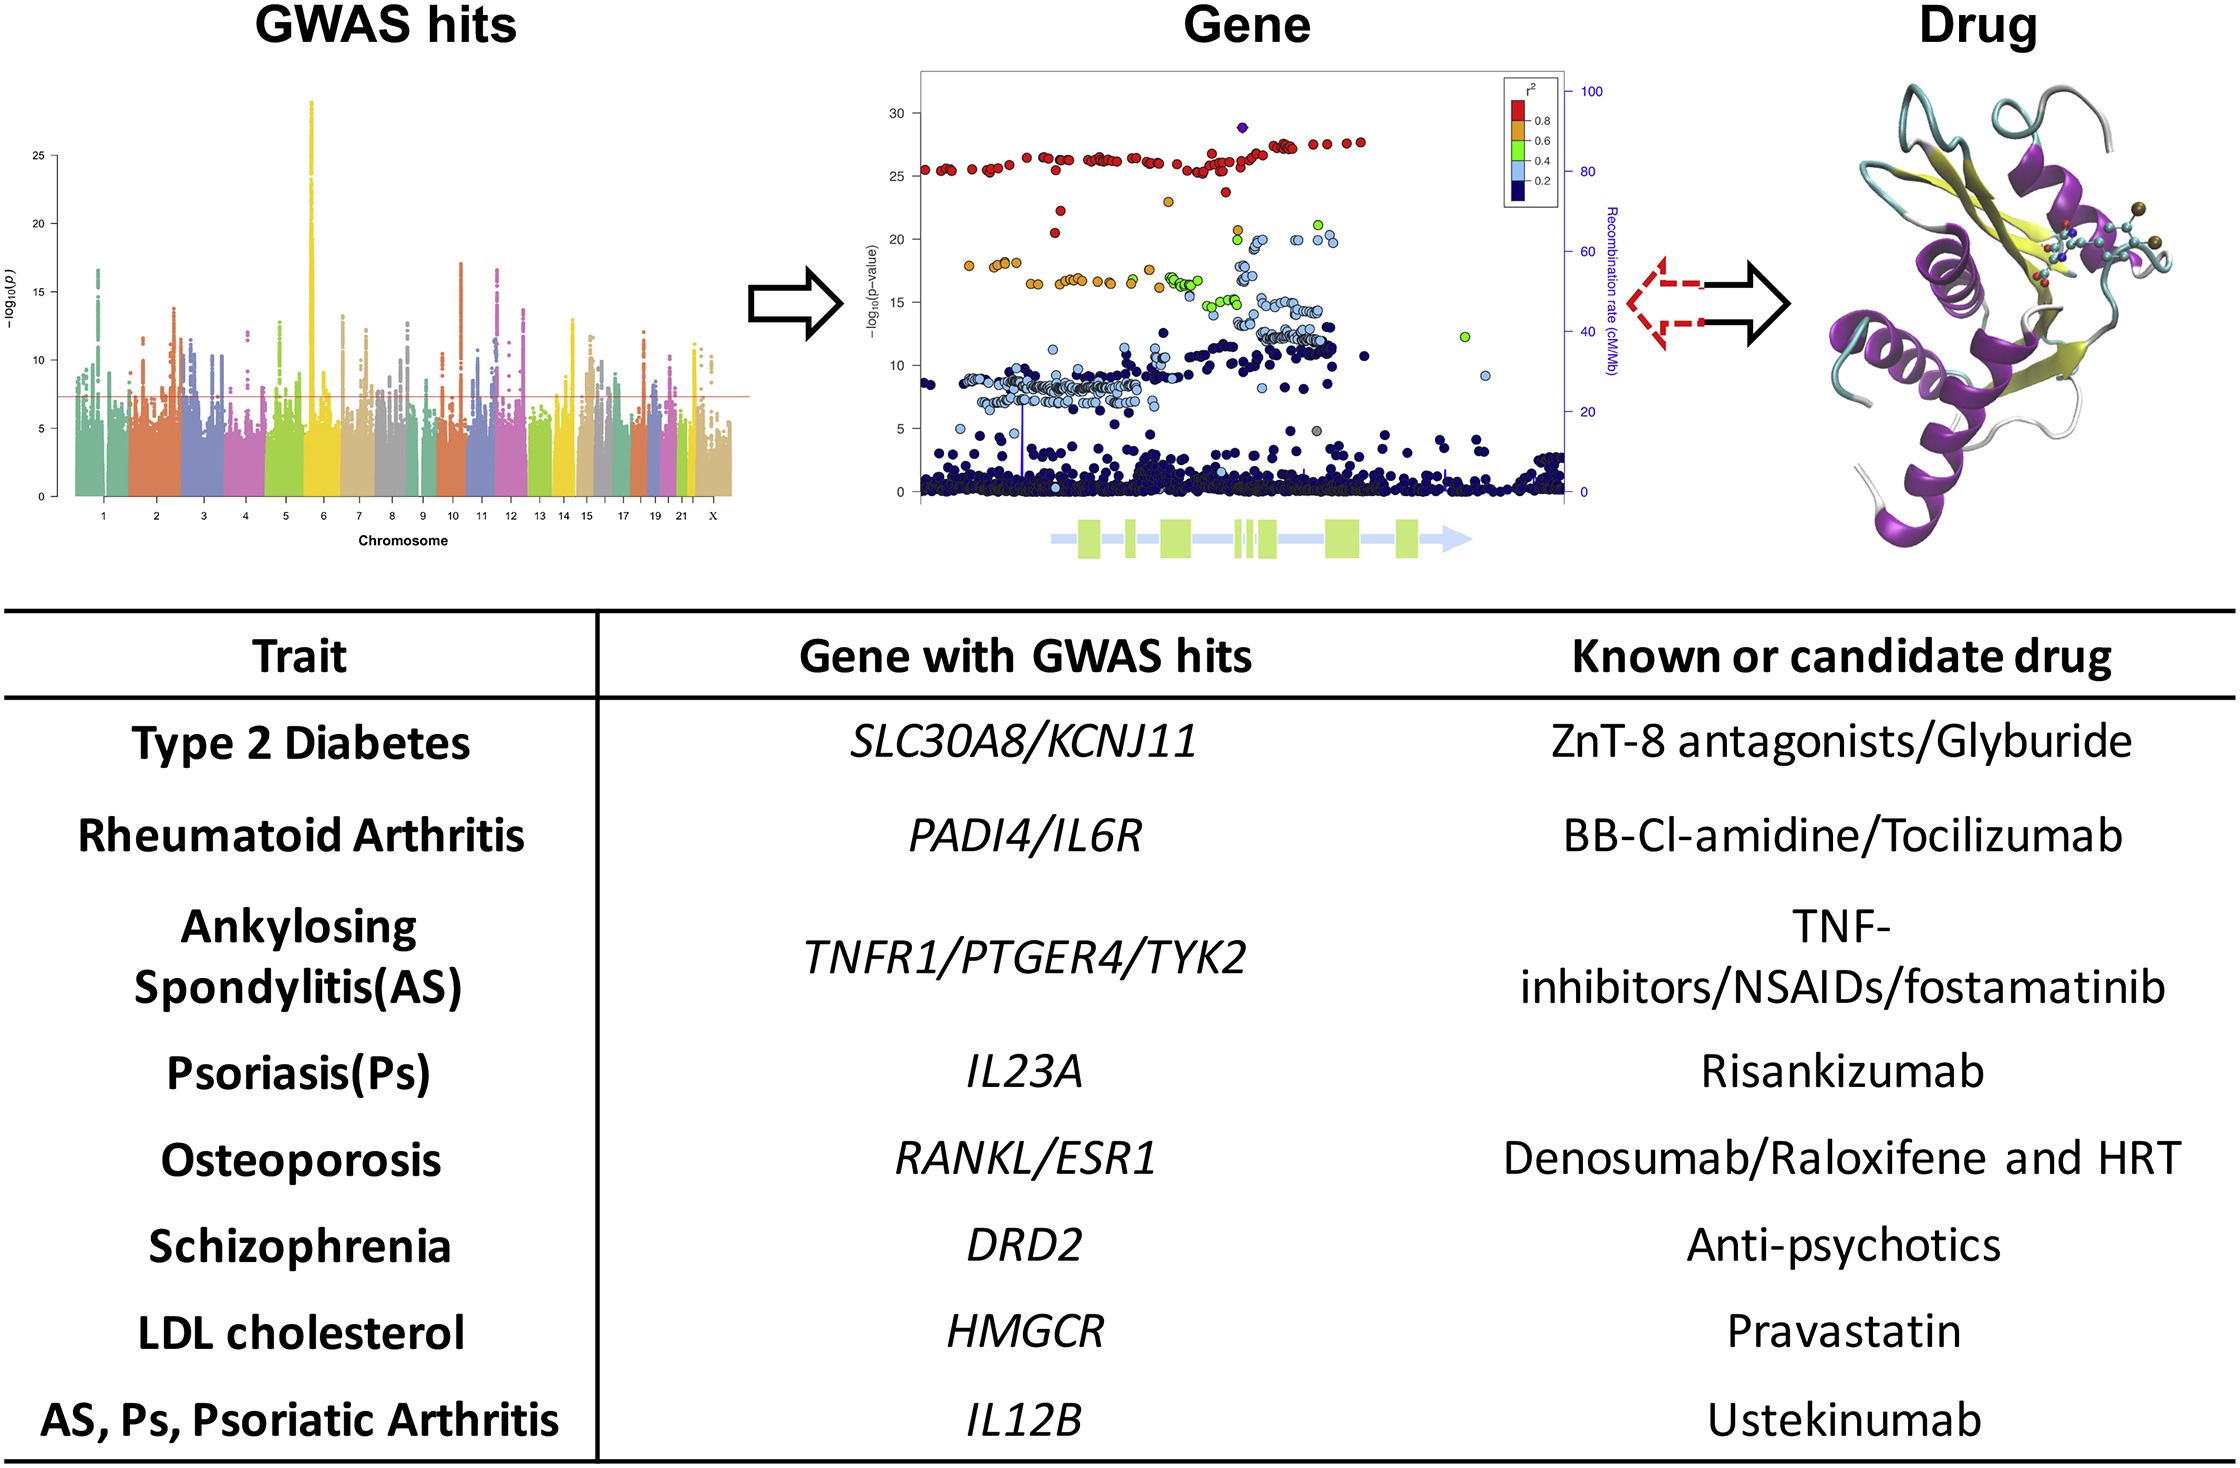
\includegraphics{introduction/gwas_success}
	\caption{Some success stories. One of the genes harbouring 
		schizophrenia-associated variants is \textit{DRD2}, a dopamine 
		receptor; once the gene was known, drugs could be developed.}
	\label{introduction/gwas_success}
\end{figure}

The genomes of closely related species do not exhibit extreme 
differences, even though the species are far apart at the phenotypic 
level; the majority of differences are found in non coding 
regions\sidenote{For instance, 80\% of human genes are shared with the 
	mouse, and 40\% of nucleotides are identical. Source: Emes et al., 
	\enquote{Comparison of the genomes of human and mouse lays the 
		foundation of genome zoology}.}, suggesting that much of the 
phenotypic differences are due to differences in how genes are 
regulated. It seems to be even more so for variations between 
individuals of the same species. The mapping of eQTL has revealed that 
gene expression, as a phenotype, is predominantly regulated in \cis, is 
quite heritable and differs in different 
populations\autocite{Gilad2008}.

It has been shown that disease-associated variants often are linked to 
eQTL\autocite{Nicolae2010}. However, in general genetic variants can 
influence a phenotype in at least three ways (\reffig{eqtl_effects}): 
chromatin modification, splicing sites alteration, and change of 
expression levels through direct mechanisms\autocite{Li2016}. Although 
most times splicing does not alter gene expression, the other mechanisms 
do, suggesting that gene expression is the most important intermediate 
link in the chain of events leading from genome to phenotype.

\begin{figure}
	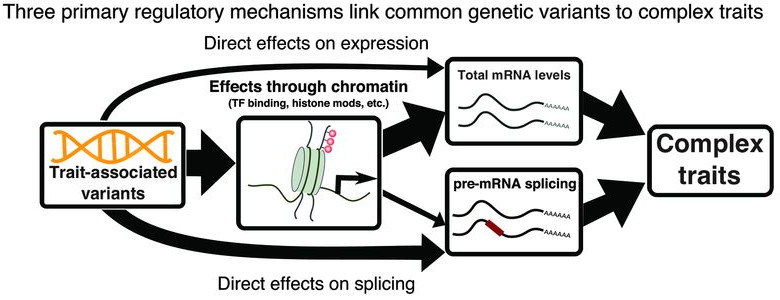
\includegraphics{introduction/eqtl_effects}
	\caption{The main effects of regulatory eQTL.}
	\label{eqtl_effects}
\end{figure}

\section{Limitations of GWAS and eQTL mapping}

The GWAS has been an important method in finding genetic variants 
associated to disease. Its integration with eQTL and functional 
annotation (mostly suggested by chromatin activity) of DNA, can provide 
and has provided valuable knowledge both for science and for clinical 
applications. Nevertheless, most variants are characterised by a small 
effect size and are not able to explain fully the 
heritability\autocite{Manolio2009}. For example, height has an 
heritability of 80\%, but the about 40 loci associated with this trait 
in 2009, after a series of GWA studies involving tens of thousands of 
people, only explained about 5\% of phenotypic variance.

Some of the causes proposed to explain this \enquote{missing 
	heritability} are the following.
\begin{itemize}
	\item Natural selection tends reduce the number of alleles 
		conferring a strong disease risk, and the remaining alleles of 
		small effect size are difficult to detect without very large 
		sample sizes.
	\item Rare variants of large effect may be present, but genotyping 
		arrays are not fully able to detect rare variants, and 
		sequencing the genomes of tens of thousand of people is 
		infeasible.
	\item Phenotypic variation might be explained by types of variation 
		different from single nucleotide polimorfisms, like CNV, but 
		genotyping arrays focus on SNPs.
	\item The effects may be due to combinations of alleles which behave 
		in a non-additive fashion; this can happen if they occur at the 
		same locus (dominance) or at different loci (epistasis).
\end{itemize}

\marginnote{Moreover, a sort of dilemma arises: to detect rare variants, 
	whole genome sequencing of a huge number of people is necessary. At 
	the same time, the differences among individuals revealed by WGS are 
	so many that trying to associate them with anything can become 
	statistically very dificult due to allelic heterogeneity. At each 
	generation, some 40 \denovo mutations per genome are introduced in 
	the population, since the mutation rate for humans is about $1.2 
	\cdot 10^{-8}$ nucleotides per genome per generation. Source of the 
	mutation rate datum: Kong et al., \enquote{Rate of de novo mutations 
		and the importance of father’s age to disease risk}.}

Another limitation of GWAS and eQTL is that, although most hits fall in 
regulatory regions and are known to have an effect on gene expression, 
these studies do not explain how the variant makes one individual more 
liable to a disease.

By exploiting the fact that most trait-associated variants influence 
gene expression, transcriptome-wide association studies aim to find 
correlations between expression and traits. Gene expression lies at an 
higher level than DNA, therefore variation in expression levels are the 
result of the combination of many genetic variants; TWAS naturally take 
account of this and aggregate the effects of many SNPs into an 
intermediate phenotype, which then is correlated to a yet higher level 
phenotype, such as a disease.

Thus, while GWAS and eQTL mapping find associations between genetic 
variants and phenotype or gene expression, respectively, TWAS find 
associations between gene expression and phenotypes. On the one hand, 
this reduces the statistical tests to perform; on the other hand, it 
increases the interpretability of results. Indeed, it is easier to 
understand the function of a gene rather than of a nucleotide.

\end{document}
